\section{Exkurs: Zusammenarbeit und Kommunikation von IT und Fachabteilungen}
\begin{frame}[c]
\begin{center}
  \textbf{Informatiker sind merkwürdig}
\end{center}
\end{frame}

\begin{frame}[c]\frametitle{Missverständnis}
  \begin{quote}
    Meine Frau trug mir auf: ``Liebling, bitte geh' zum Volg und kaufe eine Flasche Milch --- wenn sie Eier haben, kaufe sechs.''

    Ich kam mit sechs Flaschen Milch zurück.

    Sie: ``Warum zum Teufel hast Du sechs Flaschen Milch geholt?''

    Ich: ``Weil sie Eier hatten!?''
  \end{quote}
\end{frame}

\section{Exkurs: Was passiert bei der Umstellung von KIDS auf RDA?}
\begin{frame}[c]
\begin{center}
  \textbf{RDA}
\end{center}
\end{frame}

\begin{frame}[c]\frametitle{Die Umstellung von KIDS auf RDA}
  \framesubtitle{und die Ablösung der EAF10 durch GND}
    \begin{itemize}
      \item \textbf{NVZ:} Drei FTE seit Oktober allein für Schulungen
      \item \textbf{BIT:} Drei FTE seit Mai für Konzeptentwicklung, Konfigurationen, Tests, Indexierungen
      \item \textbf{diverse Abteilungen:} Teilnahme an Schulungen, Unterstützung bei Tests
    \end{itemize}
\end{frame}

\begin{frame}[c]\frametitle{Auszug aus der Aufgabenliste}
  \begin{figure}
    \begin{center}
      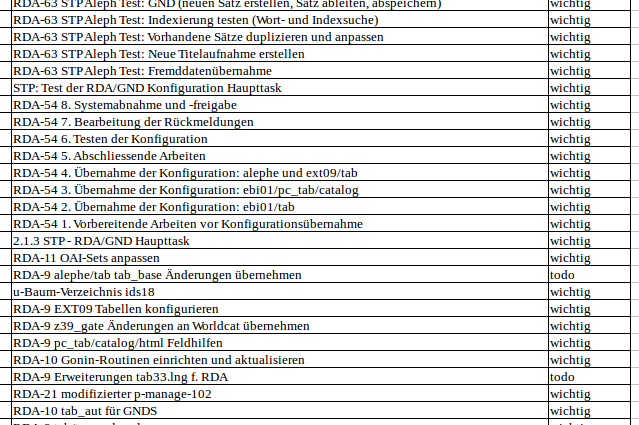
\includegraphics[width=0.8\textwidth]{pics/rda-liste}
    \end{center}
  \end{figure}
\end{frame}

\begin{frame}[c]\frametitle{Konfigurationen}  
  \begin{itemize}
    \item Das Format zum Regelwerk
    \item Automatisierungen
    \item Schnittstellen
    \item Im-- und Exportskripte
  \end{itemize}
\end{frame}

\section{Horizon Report 2015 Library Edition}
\begin{frame}[c]
\begin{center}
  \textbf{Der Horizon Report 2015 Library Edition}
\end{center}
\end{frame}

\begin{frame}[c]\frametitle{Der Horizon Report 2015 Library Edition}
    Im Horizon Report 2015 Library Edition haben sich Informations-- und Bibliotheksspezialisten Gedanken um zukünftige Entwicklungen und deren möglichen Einfluss gemacht (siehe auch: \href{http://blogs.ethz.ch/innovethbib/2015/08/24/horizon-report-2015-library-edition/}{Innovationsblog der ETH--Bibliothek}).
\end{frame}
  

\only<article>{
  Dabei geht es um drei grosse Themenkomplexe:
}

\begin{frame}[c]\frametitle<beamer>{Themen des Horizon Reports 2015 Library Edition}
    \begin{enumerate}
      \item für Forschungsbibliotheken wichtige technologische Entwicklungen
      \item Trends, die die Umsetzung beschleunigen
      \item und Herausforderungen, die diese hemmen
    \end{enumerate}
\end{frame}

 \begin{frame}    
    \frametitle{Important Developments in Technology for Academic and Research Libraries}

    \pause

      \begin{itemize}
        \item Time-to-Adoption Horizon: One Year or Less
          \begin{itemize}
            \item Makerspaces
            \item Online Learning
          \end{itemize}

        \item Time-to-Adoption Horizon: Two to Three Years
          \begin{itemize}
            \item Information Visualization
            \item Semantic Web and Linked Data
          \end{itemize}

        \item Time-to-Adoption Horizon: Four to Five Years
          \begin{itemize}
            \item Location Intelligence
            \item Machine Learning
          \end{itemize}
      \end{itemize}
  \end{frame}

  \begin{frame}
    \frametitle{Trends Accelerating Technology Adoption in Academic and Research Libraries}

    \pause

      \begin{itemize}
        \item Long-Term Impact Trends: Driving technology adoption in academic and research libraries for five or more years
          \begin{itemize}
            \item Increasing Accessibility of Research Content
            \item Rethinking Library Spaces
          \end{itemize}
        \item Mid-Term Impact Trends: Driving technology adoption in academic and research libraries over the next three to five years
          \begin{itemize}
            \item Evolving Nature of the Scholarly Record
            \item Increasing Focus on Research Data Management
          \end{itemize}
        \item Short-Term Impact Trends: Driving technology adoption in academic and research libraries over the next one to two years
          \begin{itemize}
            \item Increasing Value of the User Experience
            \item Prioritization of Mobile Content and Delivery
          \end{itemize}
      \end{itemize}
  \end{frame}
  
  \begin{frame}
    \frametitle{Challenges Impeding Technology Adoption in Academic and Research Libraries}

    \pause

      \begin{itemize}
        \item Solvable Challenges: Those that we understand and know how to solve
          \begin{itemize}
            \item Embedding Academic and Research Libraries in the Curriculum
            \item Improving Digital Literacy
          \end{itemize}
        \item Difficult Challenges: Those that we understand but for which solutions are elusive
          \begin{itemize}
            \item Competition from Alternative Avenues of Discovery
            \item Rethinking the Roles and Skills of Librarians
          \end{itemize}
        \item Wicked Challenges: Those that are complex to even define, much less address
          \begin{itemize}
            \item Embracing the Need for Radical Change
            \item Managing Knowledge Obsolescence
          \end{itemize}
      \end{itemize}
  \end{frame}

\section{Die Cloud}
\only<article>{
  Über die Cloud ist soviel Halbwissen verbreitet worden, dass ich empfehle, das Thema nochmal ganz von vorne anzudenken!
}
\begin{frame}[c]
\begin{center}
  \textbf{Die Cloud}
\end{center}
\end{frame}

\begin{frame}[c]\frametitle<beamer>{Larry Ellison über die Cloud}
    \begin{quote}
      The computer industry is the only industry, that is more fashion-driven, than women's fashion. Maybe I'm an idiot, but I have no idea what anyone is talking about. What is it? It's completely gibberish. It's insane. When is this idiocy going to stop? 
      \hfill (Larry Ellison auf der ``Oracle Open World 2008'')
    \end{quote}
\end{frame}

\only<article>{
  Grundsätzlich geht es beim Cloud---Computing um über die ganze Welt verteilte Daten und Rechenkapazitäten. Dabei spielt es durch die zusammengeschaltete Menge an Rechnern keine Rolle, wenn einzelne Systeme mehr oder weniger Leistung bringen oder gar komplett ausfallen. Auch die Daten sind so intelligent zerlegt und verteilt, dass der Ausfall eines Datencenters unerheblich ist.
  Exzellente Beispiele sind Universitätsprojekte wie seti@home oder folding@home.

  Meistens wird beim Outsourcing ein externes Rechenzentrum irrtümlich als Cloud bezeichnet. Tatsächlich bedeutet Cloud eigentlich, dass die Daten nicht mehr (ausschliesslich) im eigenen Haus liegen, aber eben nicht nur in einem Rechenzentrum, sondern verteilt auf viele.
}

\begin{frame}
  \frametitle{Services in der Cloud}
  \begin{itemize}
    \item IaaS
    \item SaaS
    \item PaaS
  \end{itemize}
\end{frame}

\only<article>{
  Larry Ellison hat vollkommen Recht: Keiner dieser Services setzt die Cloud voraus! Aber sie alle können davon proftieren. 
}

\begin{frame}[c]\frametitle{Iaas}
  \framesubtitle{Infrastructure as a Service}
  \begin{figure}
    \begin{center}
      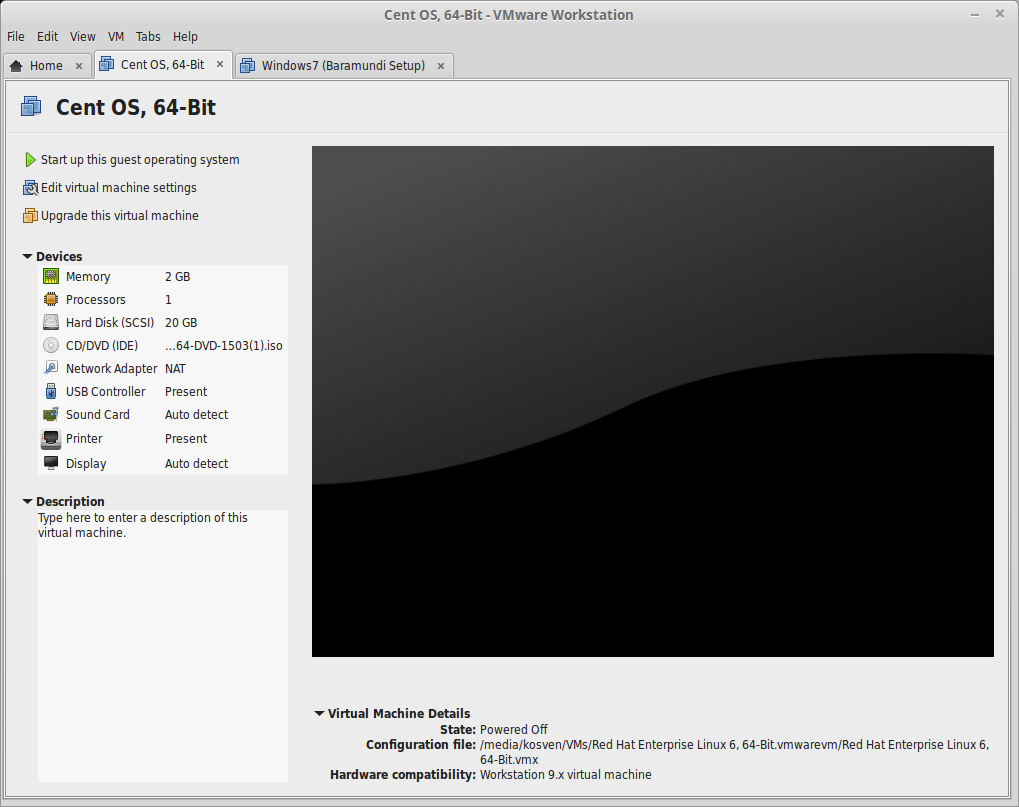
\includegraphics[width=0.6\textwidth]{pics/IaaS}
    \end{center}
  \end{figure}
\end{frame}

\begin{frame}[c]\frametitle{Saas}
  \framesubtitle{Software as a Service}
    \begin{center}
      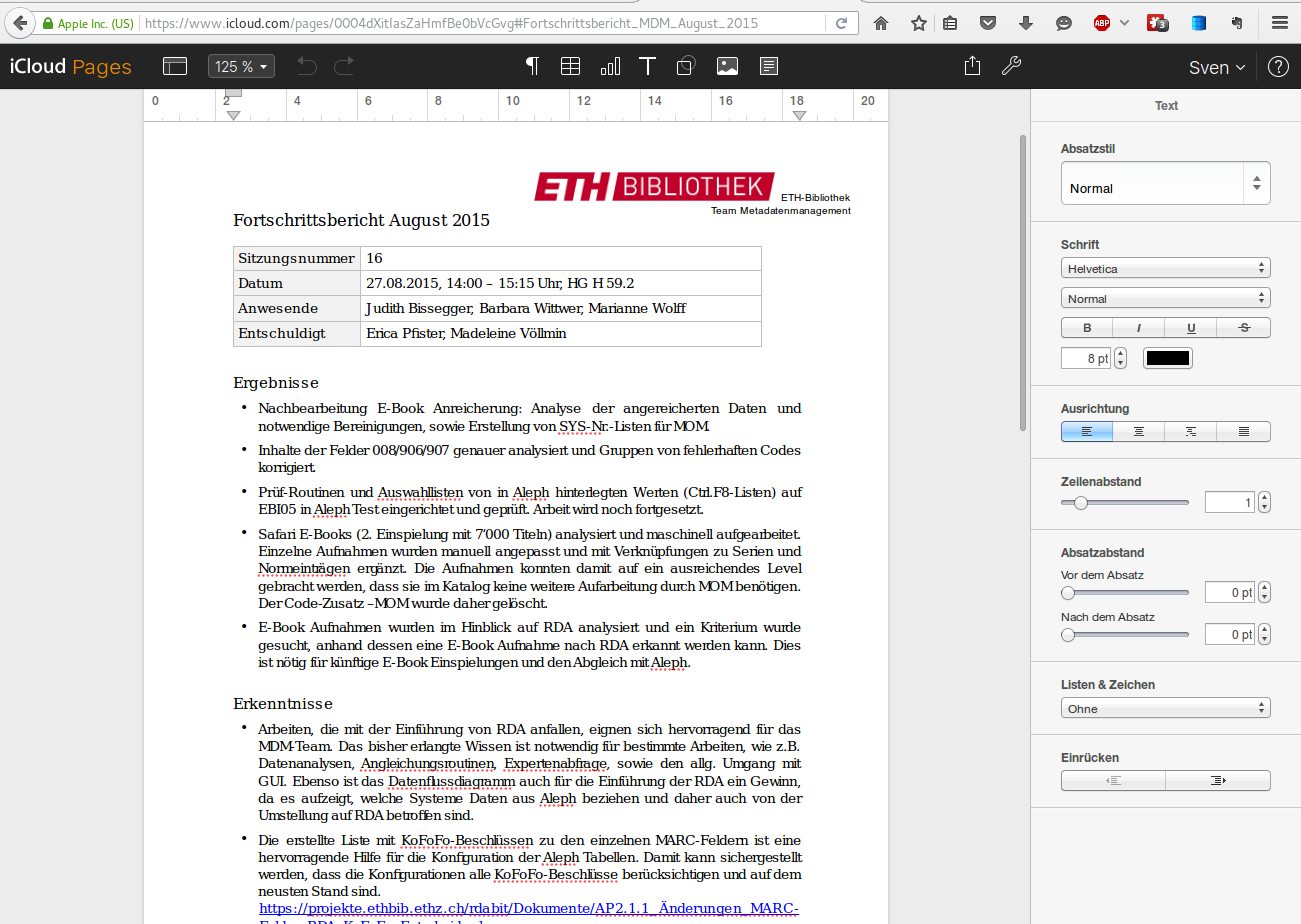
\includegraphics[width=0.8\textwidth]{pics/SaaS}
    \end{center}
\end{frame}

\begin{frame}[c]\frametitle{Paas}
  \framesubtitle{Platform as a Service}
  \begin{figure}
    \begin{center}
      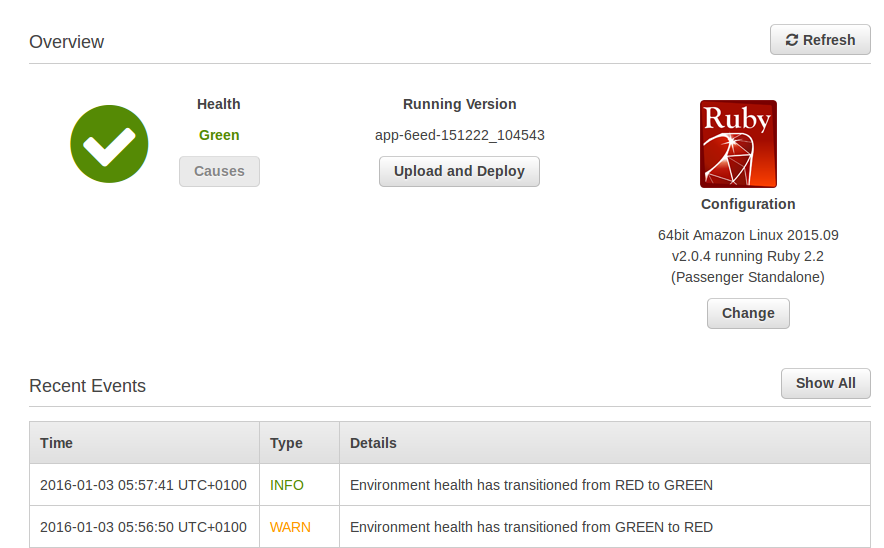
\includegraphics[width=0.8\textwidth]{pics/aws-eb}
      \caption{Beispiel: AWS: Elastic Beanstalk}
    \end{center}
  \end{figure}
\end{frame}

\section{Sicherheit}

\begin{frame}[c]
\begin{center}
  \textbf{Sicherheit in der IT}
\end{center}
\end{frame}

\begin{frame}
  \frametitle{Sicherheit}
    \begin{theorem}
      Der sichere PC steht im Tresor ohne Strom und Netzwerkanschluss.
    \end{theorem}
    \textbf{Gefahren}
    \begin{itemize}
       \item trügerische Sicherheit
       \item Halbwissen: I hacked 127.0.0.1
    \end{itemize}
\end{frame}

\begin{frame}[fragile]
  \frametitle{trügerische Sicherheit}
  \framesubtitle{Anfrage}
    \begin{lstlisting}
      Guten Tag

      Könnten Sie HTTPS für opac.nebis.ch aktivieren?
      Ich musste heute das Nebis aus dem Ausland benutzen.

      Das Login wurde zwar über https://login.library.ethz.ch/
      geschützt, dann wurde die Verschlüsselung für das 
      Ausleihen der Bücher wieder abgeschaltet.

      Je nach Land kann sogar eine Suche nach einem kritischen
      Buch zu Problemen führen.

      Darum bitte ich Sie, HTTPS auch für das Ausleihen 
      einzuschalten.
    \end{lstlisting}
\end{frame}

\begin{frame}[c]\frametitle{Halbwissen}
    \framesubtitle{I hacked 127.0.0.1}
    \begin{center}
      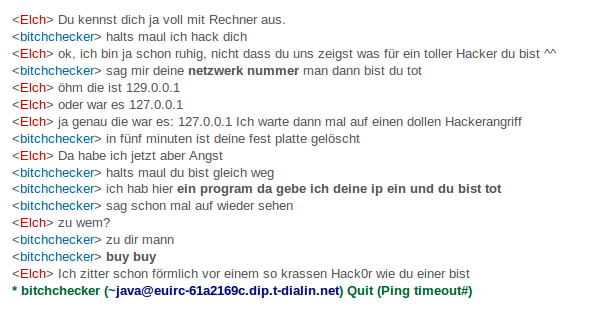
\includegraphics[width=0.8\textwidth]{pics/halbwissen}
    \end{center}
\end{frame}

\begin{frame}[c]
  \begin{quote}
    \begin{center}
      \\
      \bigskip
      \\
      {\huge Stay hungry.}
      \\
      \medskip
      \\
      {\huge Stay foolish.}
       \\
      \bigskip
      \\
      \hfill{Steve Jobs, 2005 in Stanford}
    \end{center}
  \end{quote}
\end{frame}